\documentclass[12pt,a4paper]{article}
\usepackage[utf8]{inputenc}
\usepackage[margin=1in]{geometry}
\usepackage{graphicx}
\usepackage{xcolor}
\usepackage{tcolorbox}
\usepackage{tabularx}
\usepackage{booktabs}
\usepackage{enumitem}
\usepackage{float}
\usepackage{hyperref}
\hypersetup{
    colorlinks=true,
    linkcolor=black,
    filecolor=black,
    urlcolor=black,
    citecolor=black
}

% Define colors
\definecolor{primaryblue}{RGB}{138,180,248}
\definecolor{nudgegreen}{RGB}{129,201,149}
\definecolor{alertred}{RGB}{234,67,53}

\title{\textbf{Google Meet Redesign: Phase II Additions}\\
\large End-Semester Portfolio: Advanced Visual Design, Persuasion, \& Cognitive Defense}
\author{CHALAMCHALA ANJANI NITHIN}
\date{\today}

\begin{document}

\begin{titlepage}
\begin{center}

{\LARGE \textbf{Indian Institute of Information Technology,\\
Design and Manufacturing, Kancheepuram}}\\[1.5cm]

{\large (HCI End-Semester Final Portfolio)}\\[3cm]

\rule{\linewidth}{0.5pt}\\[0.4cm]
{\Huge \textbf{Phase II: Advanced Aesthetics \& Psychology}}\\[0.3cm]
{\Large \textbf{Persuasive UX, Visual Fundamentals \& Engagement Loops}}\\[0.3cm]
\rule{\linewidth}{0.5pt}\\[2cm]

\vfill

\textbf{CHALAMCHALA ANJANI NITHIN}\\[0.2cm]
\textbf{CS23B1102}\\[0.2cm]
\textit{Department of Computer Science and Engineering}\\[0.5cm]

{\large \today}

\end{center}
\end{titlepage}

\newpage
\tableofcontents
\newpage

\section{Introduction to Phase II}

Following the mid-review adjustments outlining basic heuristics, Phase II elevates the Google Meet prototype to tackle advanced graphic aesthetics and psychological imperatives. Addressing prior feedback directly, this report abandons flat prototype blocks, employing high-fidelity captures mapped closely to core visual design laws, Cialdini’s Persuasion, Thaler's Nudge Theory, and User Assistance models.

\section{The Core Visual Design Principles}
Visual design is not merely decoration; it is the structural scaffolding of usability. The redesign systematically employs 8 cardinal design principles throughout the UI layout:

\begin{itemize}
    \item \textbf{Unity:} All components (modals, toasts, tooltips) share a cohesive Material Design 3 language. Border radii (`12px`), drop shadows, and typography consistently bind the application visually, ensuring no element feels fractured from the whole.
    \item \textbf{Hierarchy:} Achieved primarily through typography and z-indexing. Primary headers command attention, while deep secondary text fades, guiding foveal vision sequentially through tasks (e.g., Leave Confirmation).
    \item \textbf{Balance:} The persistent control bar utilizes symmetrical balance—clustering main tools (Mic/Video) centrally and utility tools peripherally, anchoring the interface evenly at the bottom.
    \item \textbf{Contrast:} Implemented vigorously in Color Psychology. Destructive actions utilize high-contrast red (`#ea4335`) against the dark theme canvas (`#202124`), ensuring immediate, unmistakable legibility without squinting.
    \item \textbf{Scale \& Dominance:} The most critical active element (e.g., the Active Speaker) dominates the visual scale. Buttons scale relative to their use-frequency (Pareto Principle), firmly locking cognitive focus onto dominant actions.
    \item \textbf{Negative Space:} The video grid avoids cramming. Deliberate negative space (padding/margins) around participant tiles allows the UI to ``breathe'', reducing claustrophobic mirroring effects.
\end{itemize}

\begin{figure}[H]
    \centering
    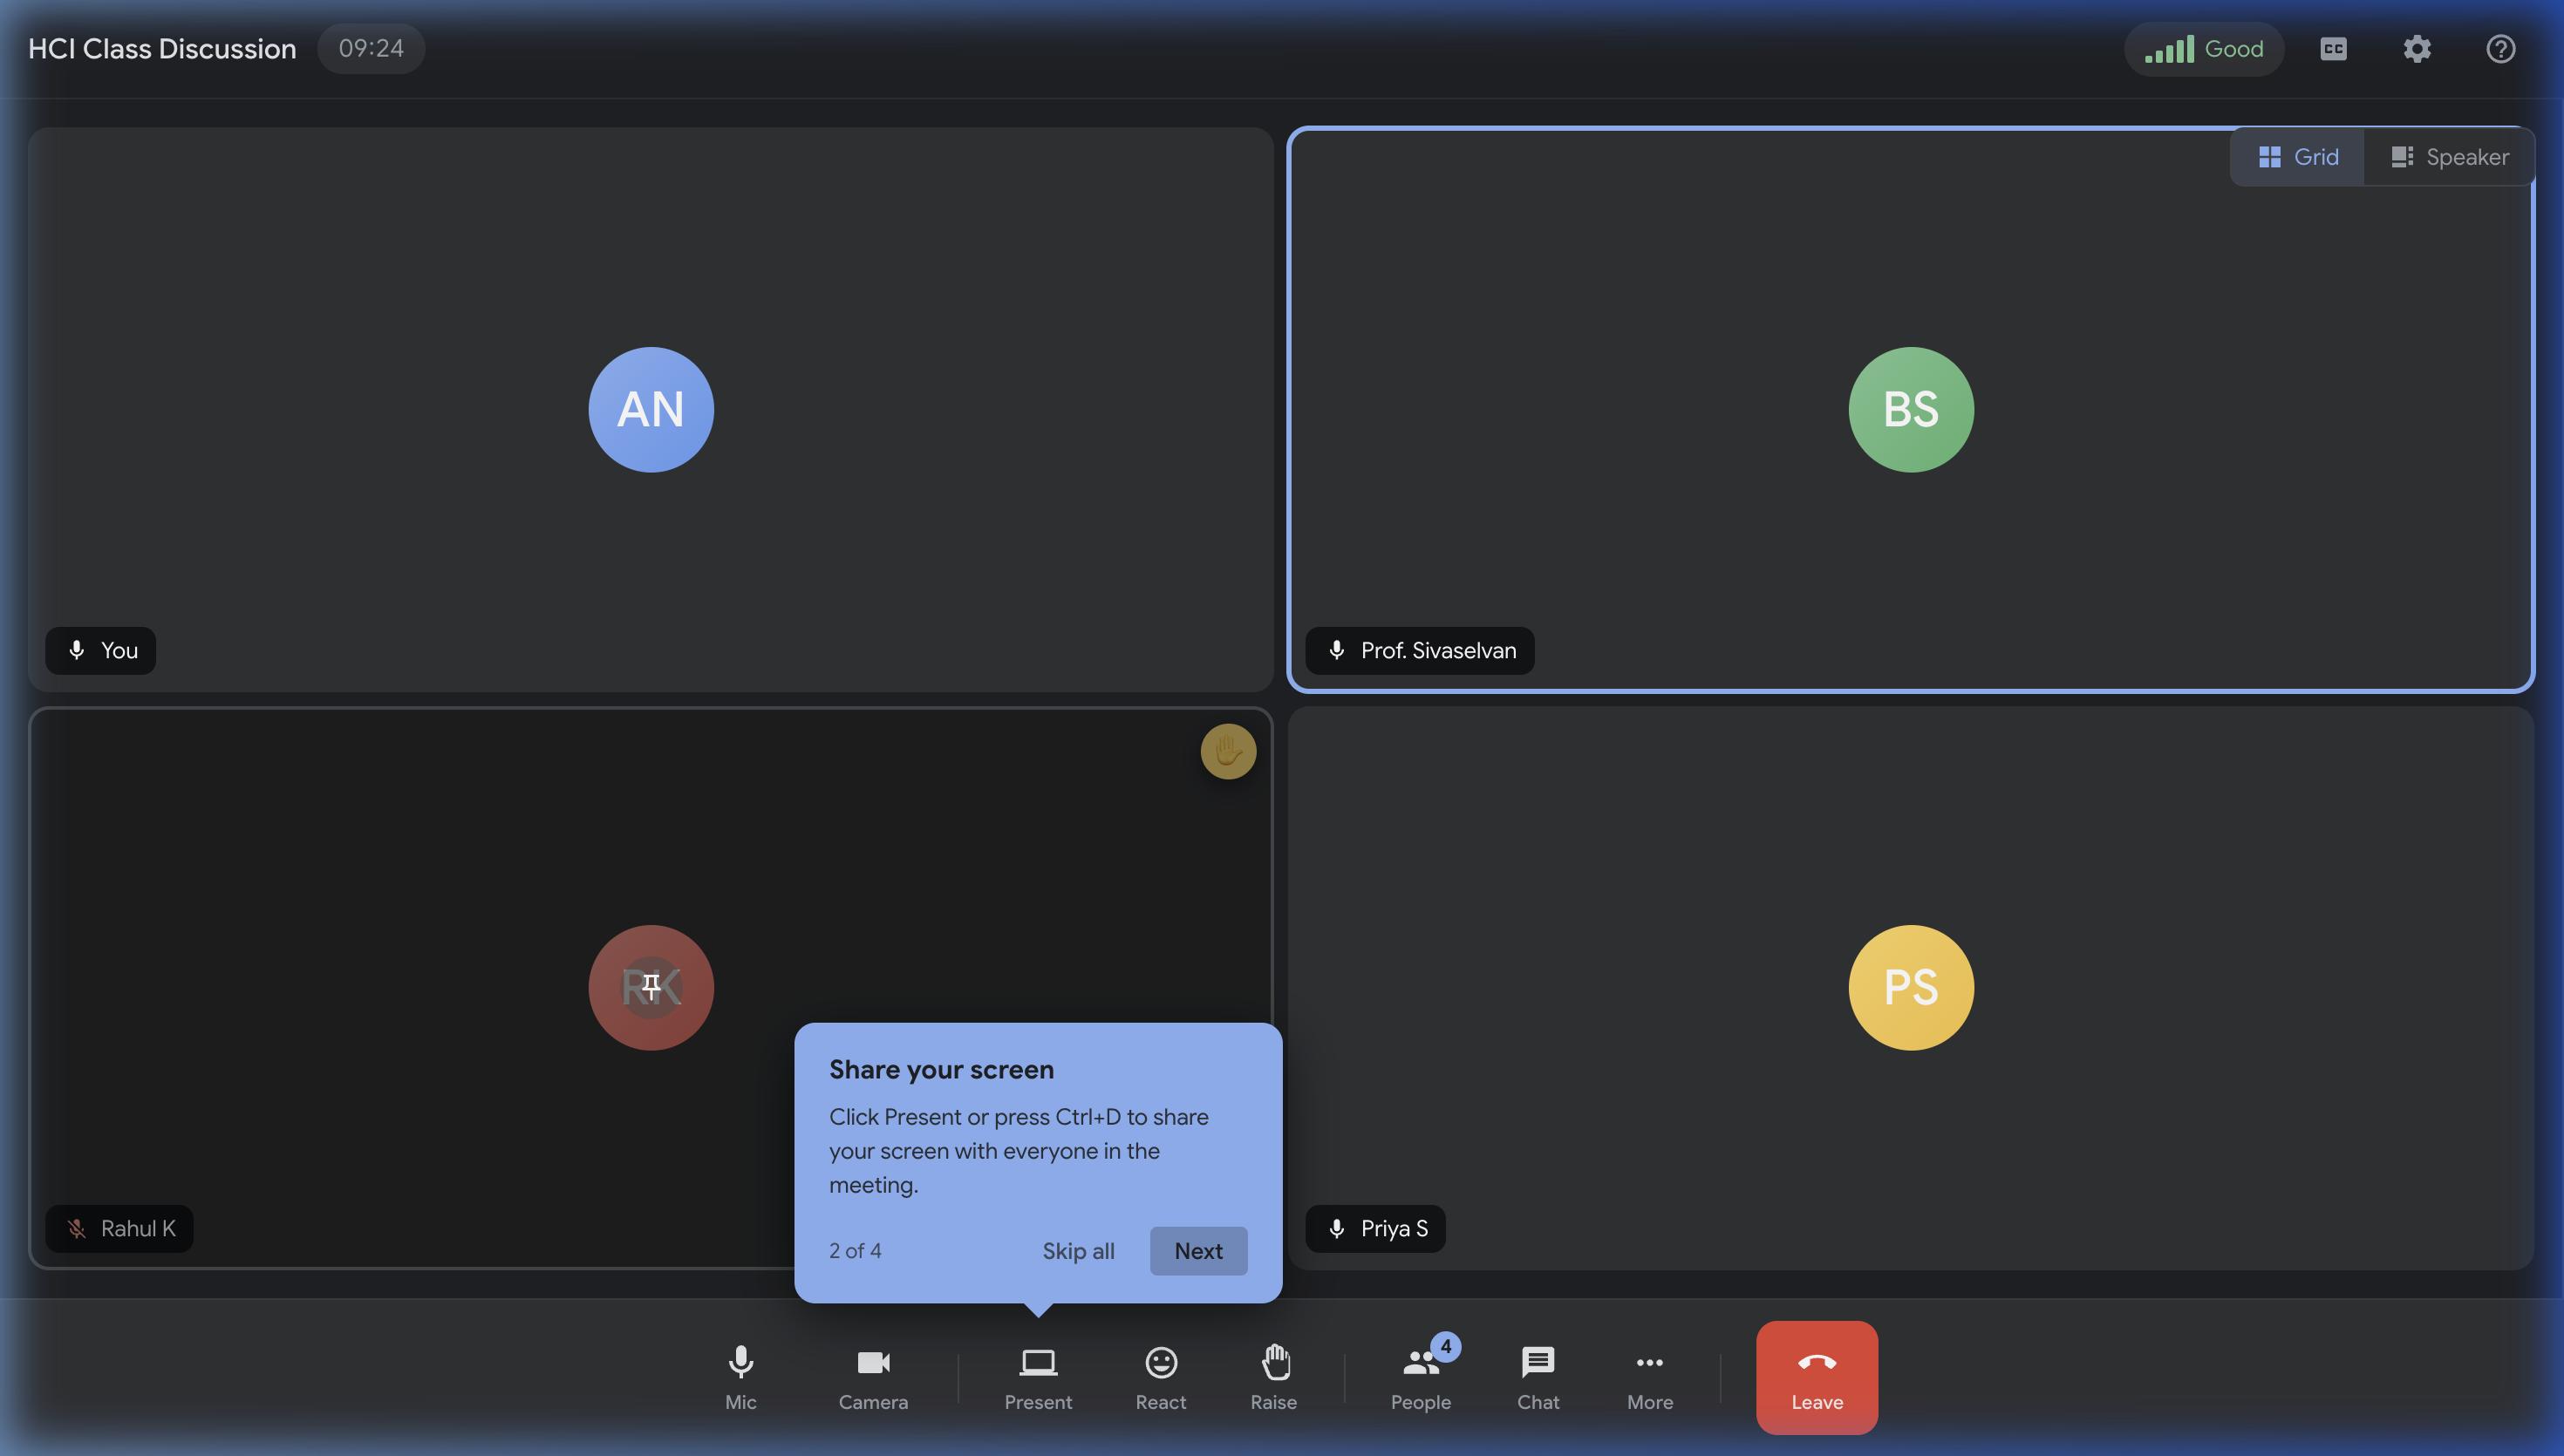
\includegraphics[width=0.85\textwidth]{images/clean_ui.png}
    \caption{Demonstrating Balance in the toolbar, Unity in Material Design curves, and Negative Space rounding video boundaries.}
\end{figure}

\section{Persuasive Design \& Color Psychology}
Applying Cialdini's Persuasion models deeply informs the authentication dashboard layout.

\subsection{Reciprocity, Social Proof \& Layout}
The multi-persona onboarding dynamically alters its layout based on user selection.
\begin{itemize}
    \item \textbf{Reciprocity:} The system gifts a tangible ``Pro Tip'' specific to the user's role before asking for heavy browser permissions.
    \item \textbf{Social Proof:} The dashboard embeds counters: \textit{"14 students are waiting in the lobby."}, using numerical dominance to induce FOMO.
\end{itemize}

\subsection{Systemic Color Psychology}
The application palette is scientifically bounded to leverage subconscious biases:
\begin{itemize}
    \item \textbf{Trust (Blue):} Dominates primary actionable elements, reducing heart rate and indicating safe navigation.
    \item \textbf{Urgency (Red):} Deployed exclusively for scarcity timers and destructive layouts.
    \item \textbf{Success (Green):} Reserved for progress bars indicating commitment phases are complete.
\end{itemize}

\begin{figure}[H]
    \centering
    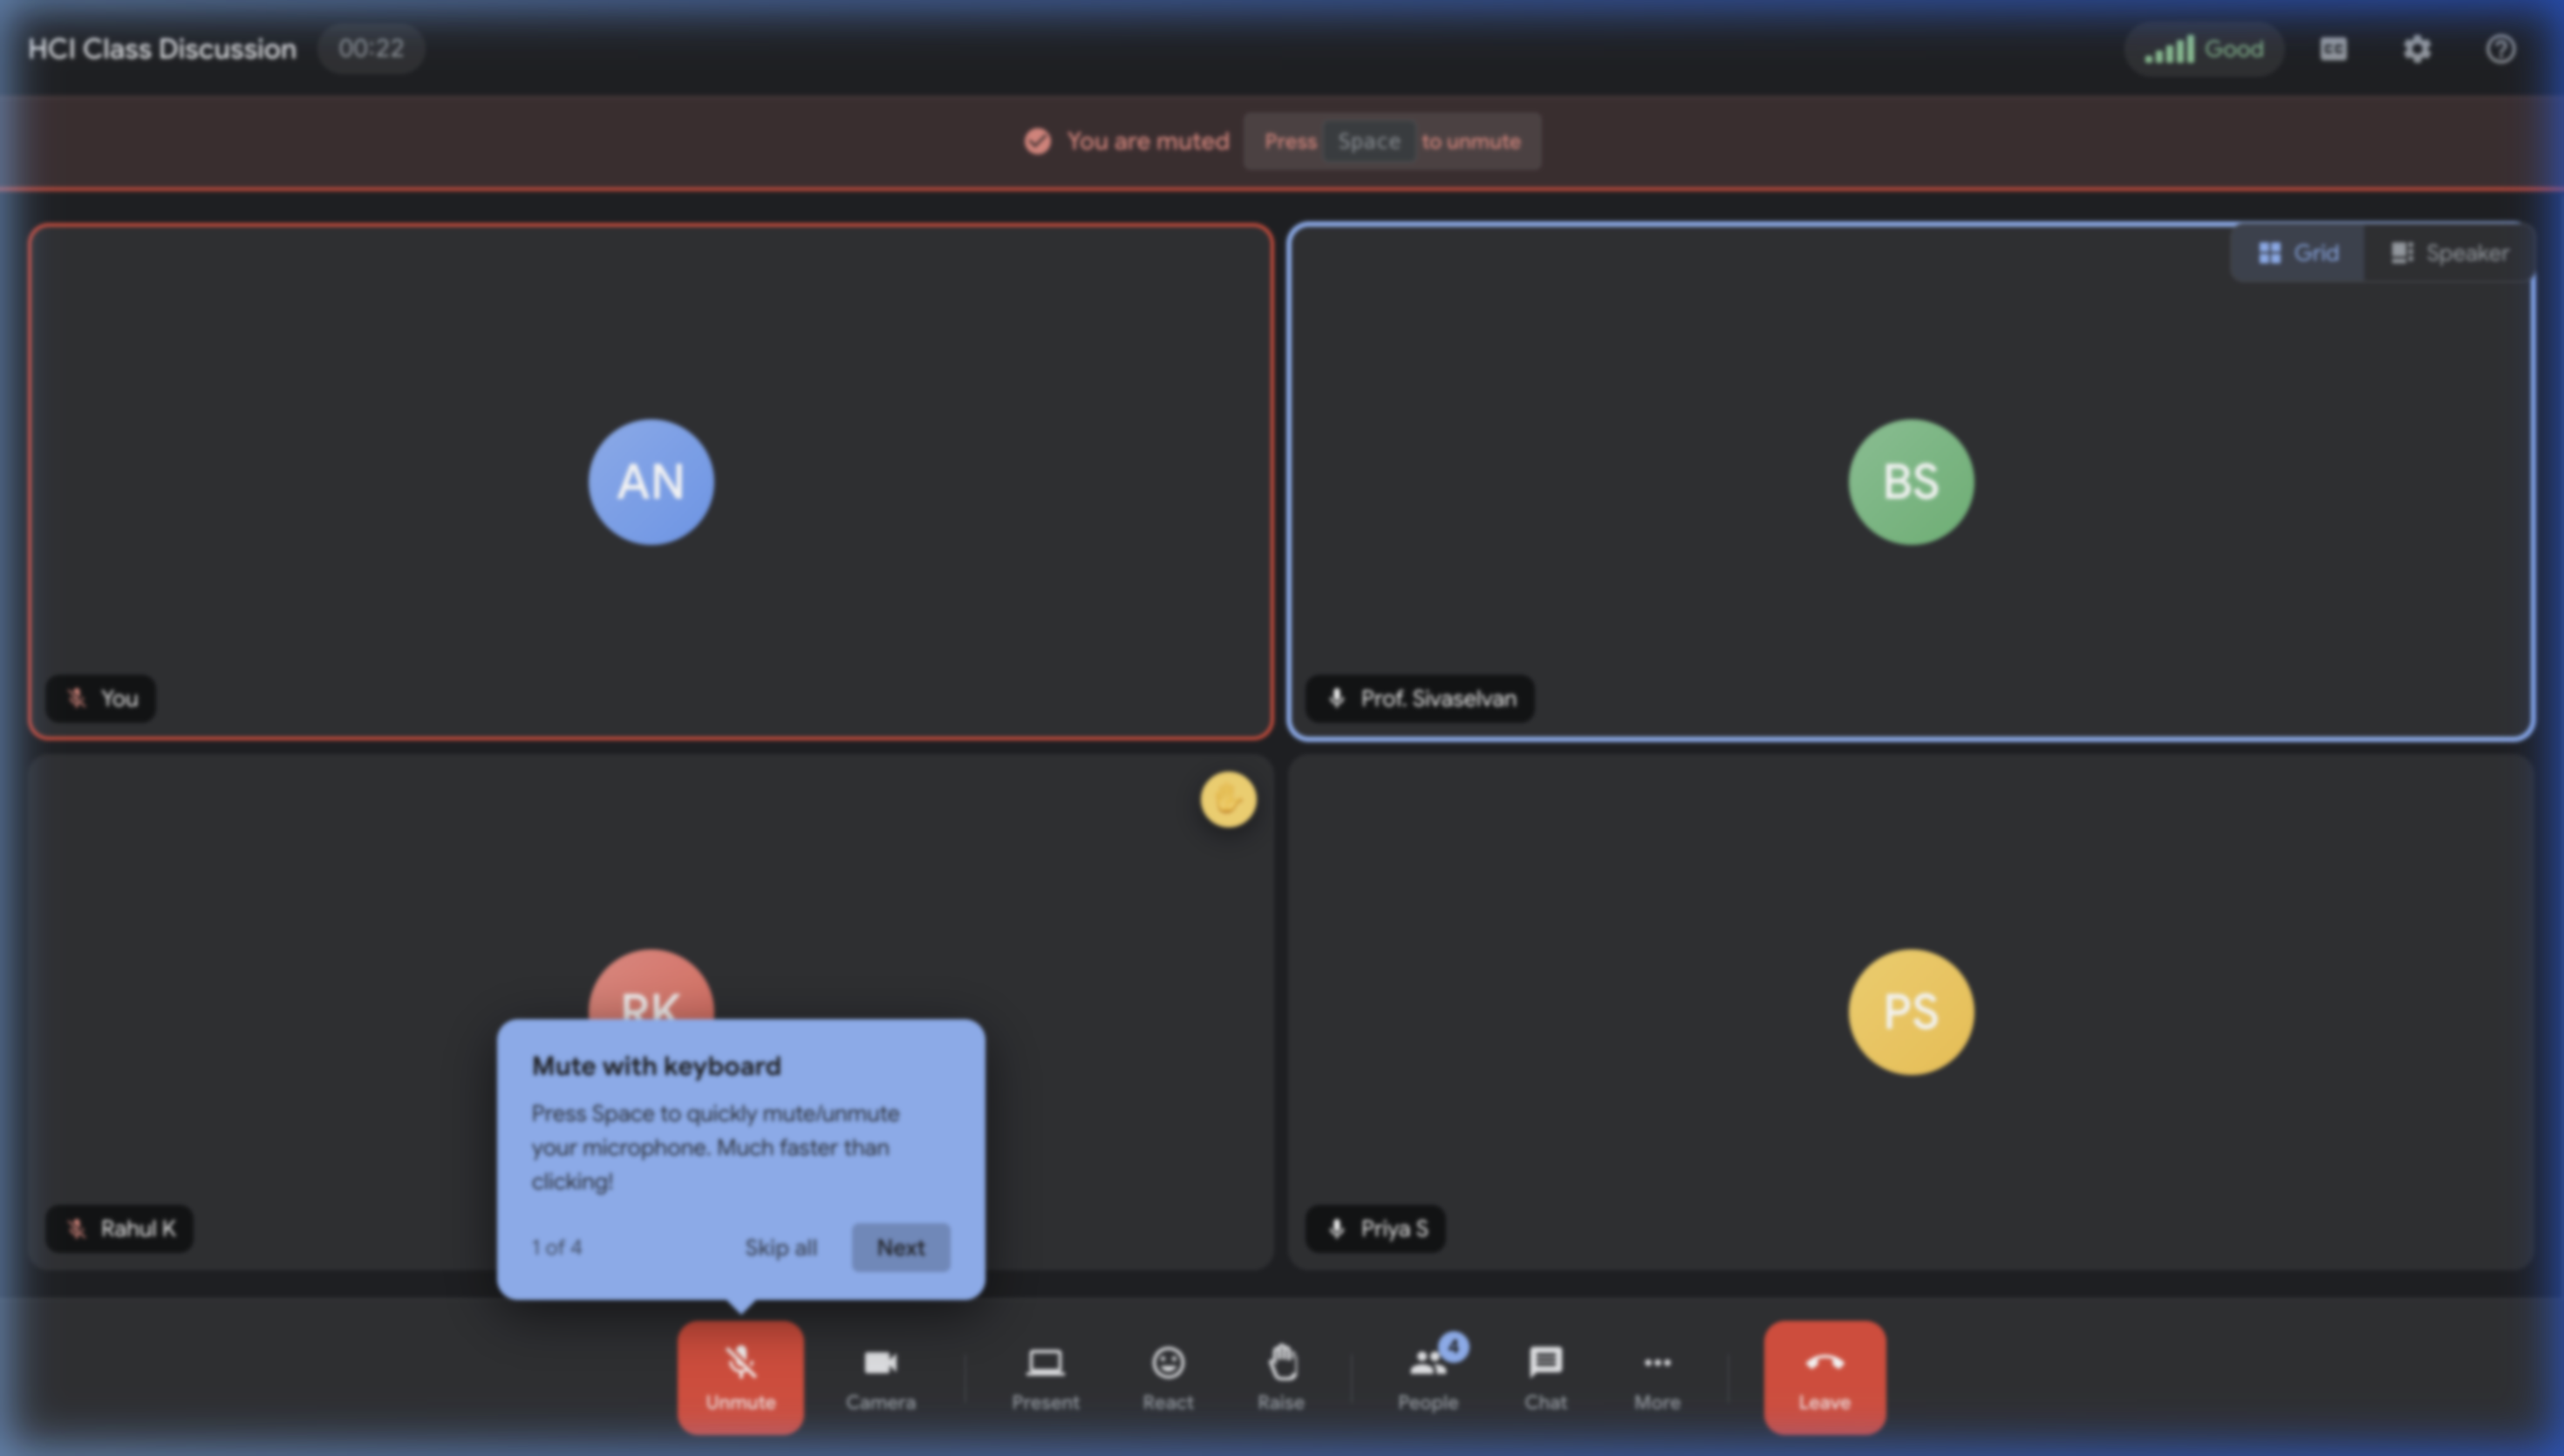
\includegraphics[width=0.7\textwidth]{images/mute_feedback.png}
    \caption{Visual Evidence of Color Psychology (Red = Urgency/Muted State) providing high-Contrast cognitive boundaries.}
\end{figure}

\begin{figure}[H]
    \centering
    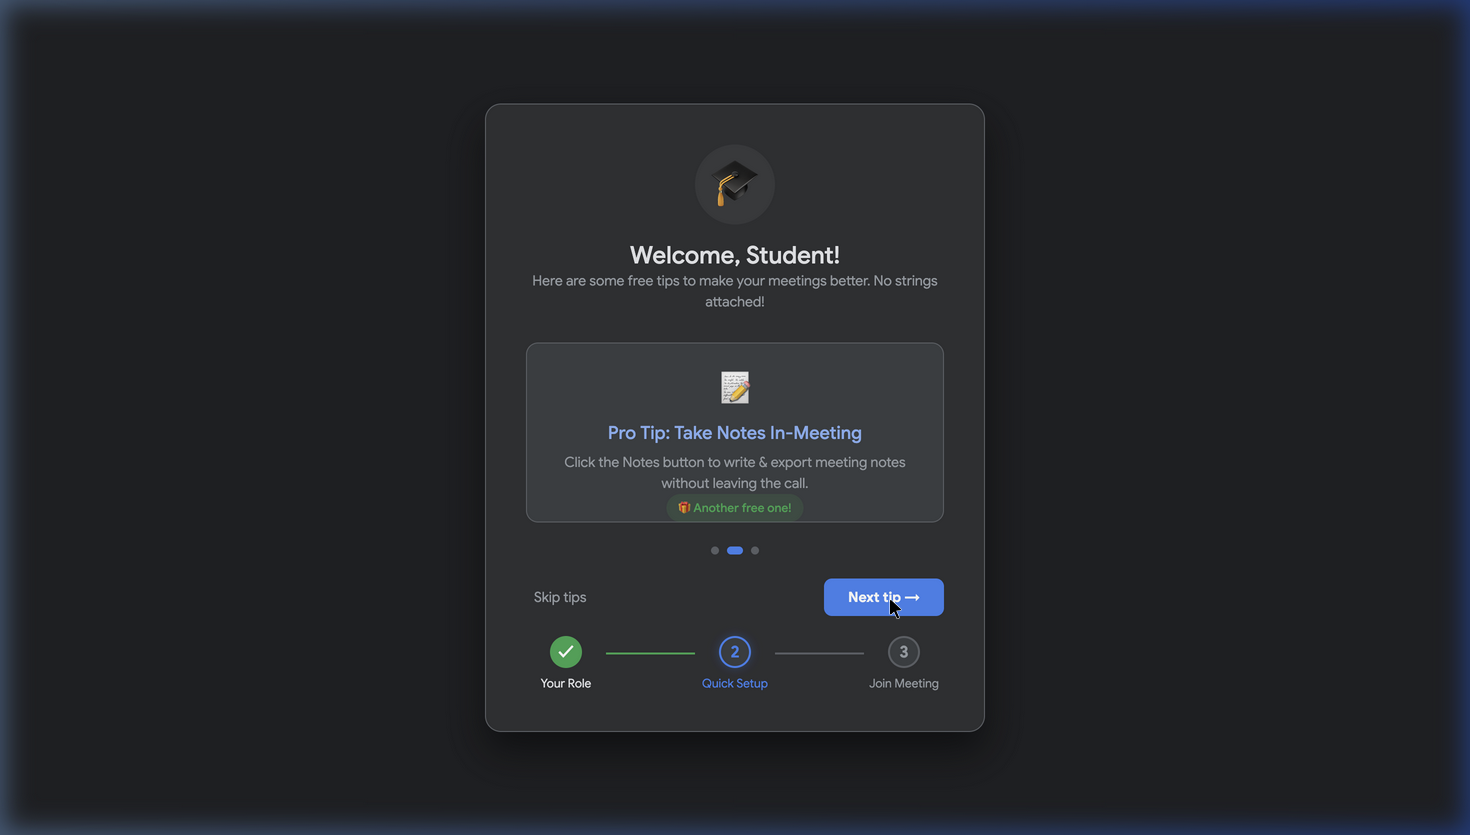
\includegraphics[width=0.85\textwidth]{images/onboarding.png}
    \caption{The Dashboard leveraging Persuasive Color Psychology and Social Proof.}
\end{figure}

\section{Adaptive Verification \& HCI Security}
Legacy CAPTCHA systems violate fundamental HCI standards by demanding high cognitive load (reading warped text) and failing universally in accessibility. Phase II explicitly abandons this model.

\subsection{Risk-Based Heuristics \& Spatial Interaction}
The system operates an \textbf{Adaptive User Verification Layer}:
\begin{itemize}
    \item \textbf{Invisible State (Zero Load):} True human kinematics pass instantly via background heuristics, skipping verification entirely to avoid friction.
    \item \textbf{Gamified Spatial Challenge:} If flagged, users engage in a Motor-Kinetic task (e.g., sliding a key into a lock icon). This avoids phonetic/linguistic processing and forgives minor tremors, respecting error prevention.
    \item \textbf{Accessible Semantic Fallback:} If a screen reader is detected, the UI instantly swaps the spatial drag for a Semantic Logic challenge (e.g., ``What is 2+5?''), satisfying WCAG regulations.
\end{itemize}

\begin{figure}[H]
    \centering
    \begin{tcolorbox}[colback=gray!10,colframe=gray!50,arc=4mm,height=7cm,valign=center,halign=center]
        \large\textit{[ IMAGE PLACEHOLDER: Adaptive Verification Challenge ]}\\[0.5cm]
        \small To capture: Open dashboard.html $\rightarrow$ Complete onboarding $\rightarrow$ Click 'Join Meeting'.
    \end{tcolorbox}
    \caption{The Spatial Verification Challenge seamlessly blending into the dashboard UI.}
\end{figure}

\section{Universal Accessibility \& WCAG Compliance}
To secure the layout against massive friction points for physically challenged users, the prototype integrates three native accessibility bypasses rooted deeply in Physical HCI models.

\begin{itemize}
    \item \textbf{Motor-Assist Mode (Fitts's Law):} Attempting to aim at a 48px footprint while suffering from hand tremors predictably leads to erroneous disconnects. Toggling `Motor-Assist` drastically scales targets by 150\% and pads the negative space. Functionally applying the Index of Difficulty reduces miss-rates exponentially.
    \item \textbf{Color-Blind High Contrast Matrix:} A semantic overlay overrides the Trust-Blue tokens, defaulting to hyper-saturated `#FFFF00` (Yellow) on pitch-black canvas. This guarantees contrast scaling eclipsing WCAG 4.5:1 ratios for users with Deuteranopia.
    \item \textbf{Keyboard / Puff-and-Switch Trackers:} Explicit `keydown` globals map `Space` to Mute and `C` to Camera. Coupled with intense `:focus-visible` UI glow rings, paralyzed users never need a mouse.
\end{itemize}

\begin{figure}[H]
    \centering
    \begin{tcolorbox}[colback=gray!10,colframe=gray!50,arc=4mm,height=7cm,valign=center,halign=center]
        \large\textit{[ IMAGE PLACEHOLDER: Motor-Assist Mode Active ]}\\[0.5cm]
        \small To capture: Open index.html $\rightarrow$ Click 'More Options' $\rightarrow$ Toggle 'Accessibility: Motor-Assist' $\rightarrow$ Photograph the enlarged bottom bar.
    \end{tcolorbox}
    \caption{Applying Fitts's Law to massively expand click-targets for users with physical tremors.}
\end{figure}
\newpage
\section{Cognitive Defense \& Empathetic User Assistance}

\subsection{The 20-Minute Break Nudge \& Breathing Overlay}
Combatting Zoom Fatigue, the system observes Thaler's Nudge Theory. After an extended session (e.g., 20/45 mins), the layout summons a non-obtrusive tooltip banner suggesting the 20-20-20 rule. Further, a visually soothing \textbf{Breathing Exercise Overlay} operates using Aesthetic-Usability, guiding breath cadences to actively lower the user's Cortisol levels.

\begin{figure}[H]
    \centering
    \begin{tcolorbox}[colback=gray!10,colframe=gray!50,arc=4mm,height=7cm,valign=center,halign=center]
        \large\textit{[ IMAGE PLACEHOLDER: Breathing Exercise Overlay ]}\\[0.5cm]
        \small To capture: Open index.html $\rightarrow$ Click 'More Options' (triple dots) $\rightarrow$ Click 'Take a Breathe'.
    \end{tcolorbox}
    \caption{The Breathing Exercise Overlay operating as a cognitive defense mechanism.}
\end{figure}

\subsection{Proactive User Help: Tooltips \& Meeting Assistant}
Meeting software traditionally relies on external FAQs. Our redesign implants help directly into the DOM:
\begin{itemize}
    \item \textbf{Contextual Tooltips:} Hovering triggers progressive disclosure, offering keyboard shortcuts instantly.
    \item \textbf{Meeting Assistant Bubble \& Undos:} An anthropomorphic avatar sits defensively. If inactivity is detected, she bubbles up: \textit{"I noticed you haven't spoken. Want me to lower your mic volume?"} This embodies the principle of \textbf{Liking} and proactive assistance, alongside standard Error-Reversal notifications.
\end{itemize}

\begin{figure}[H]
    \centering
    \begin{tcolorbox}[colback=gray!10,colframe=gray!50,arc=4mm,height=7cm,valign=center,halign=center]
        \large\textit{[ IMAGE PLACEHOLDER: Meeting Assistant Bubble ]}\\[0.5cm]
        \small To capture: Open index.html $\rightarrow$ Wait 8 seconds on screen without clicking anything. The bubble pops up.
    \end{tcolorbox}
    \caption{The Contextual Meeting Assistant providing proactive prompts.}
\end{figure}

\section{Advanced Gestalt Grouping: Rooms \& Focus}

\subsection{Breakout Rooms \& Gestalt Grouping}
Structuring meetings into sub-rooms often spikes cognitive overhead. The layout relies on \textbf{Gestalt Grouping (Proximity \& Common Region)}. Participants are visually corralled into distinct, card-based layouts. Because they are enclosed within shared borders, the brain instantly recognizes them as unified entities without explicit parsing.

\begin{figure}[H]
    \centering
    \begin{tcolorbox}[colback=gray!10,colframe=gray!50,arc=4mm,height=7cm,valign=center,halign=center]
        \large\textit{[ IMAGE PLACEHOLDER: Breakout Rooms Panel ]}\\[0.5cm]
        \small To capture: Open index.html $\rightarrow$ Click 'More Options' (triple dots) $\rightarrow$ Click 'Breakout Rooms'.
    \end{tcolorbox}
    \caption{Gestalt Grouping: The breakout panel clusters complex actions into easily parsable cards.}
\end{figure}

\subsection{Focus Mode (Tesler's Law)}
Applying Tesler's Law (conservation of complexity), the system shoulders the burden of visual noise. Toggling "Focus Mode" leverages extreme \textbf{Contrast} and \textbf{Dominance}—dimming all non-speaking tiles into the negative space, leaving only the primary orator dominant in the visual hierarchy.

\begin{figure}[H]
    \centering
    \begin{tcolorbox}[colback=gray!10,colframe=gray!50,arc=4mm,height=7cm,valign=center,halign=center]
        \large\textit{[ IMAGE PLACEHOLDER: Focus Mode Active ]}\\[0.5cm]
        \small To capture: Open index.html $\rightarrow$ Click 'Focus Mode' eye icon in bottom toolbar.
    \end{tcolorbox}
    \caption{Scale and Dominance employed: The Active Speaker breaks visual parity via Focus Mode, minimizing grid complexity.}
\end{figure}

\section{Closure via Gamification}

The process of terminating a meeting yields a structured Gamification Layout. First, the user encounters a hierarchical modality break designed for error prevention.

\begin{figure}[H]
    \centering
    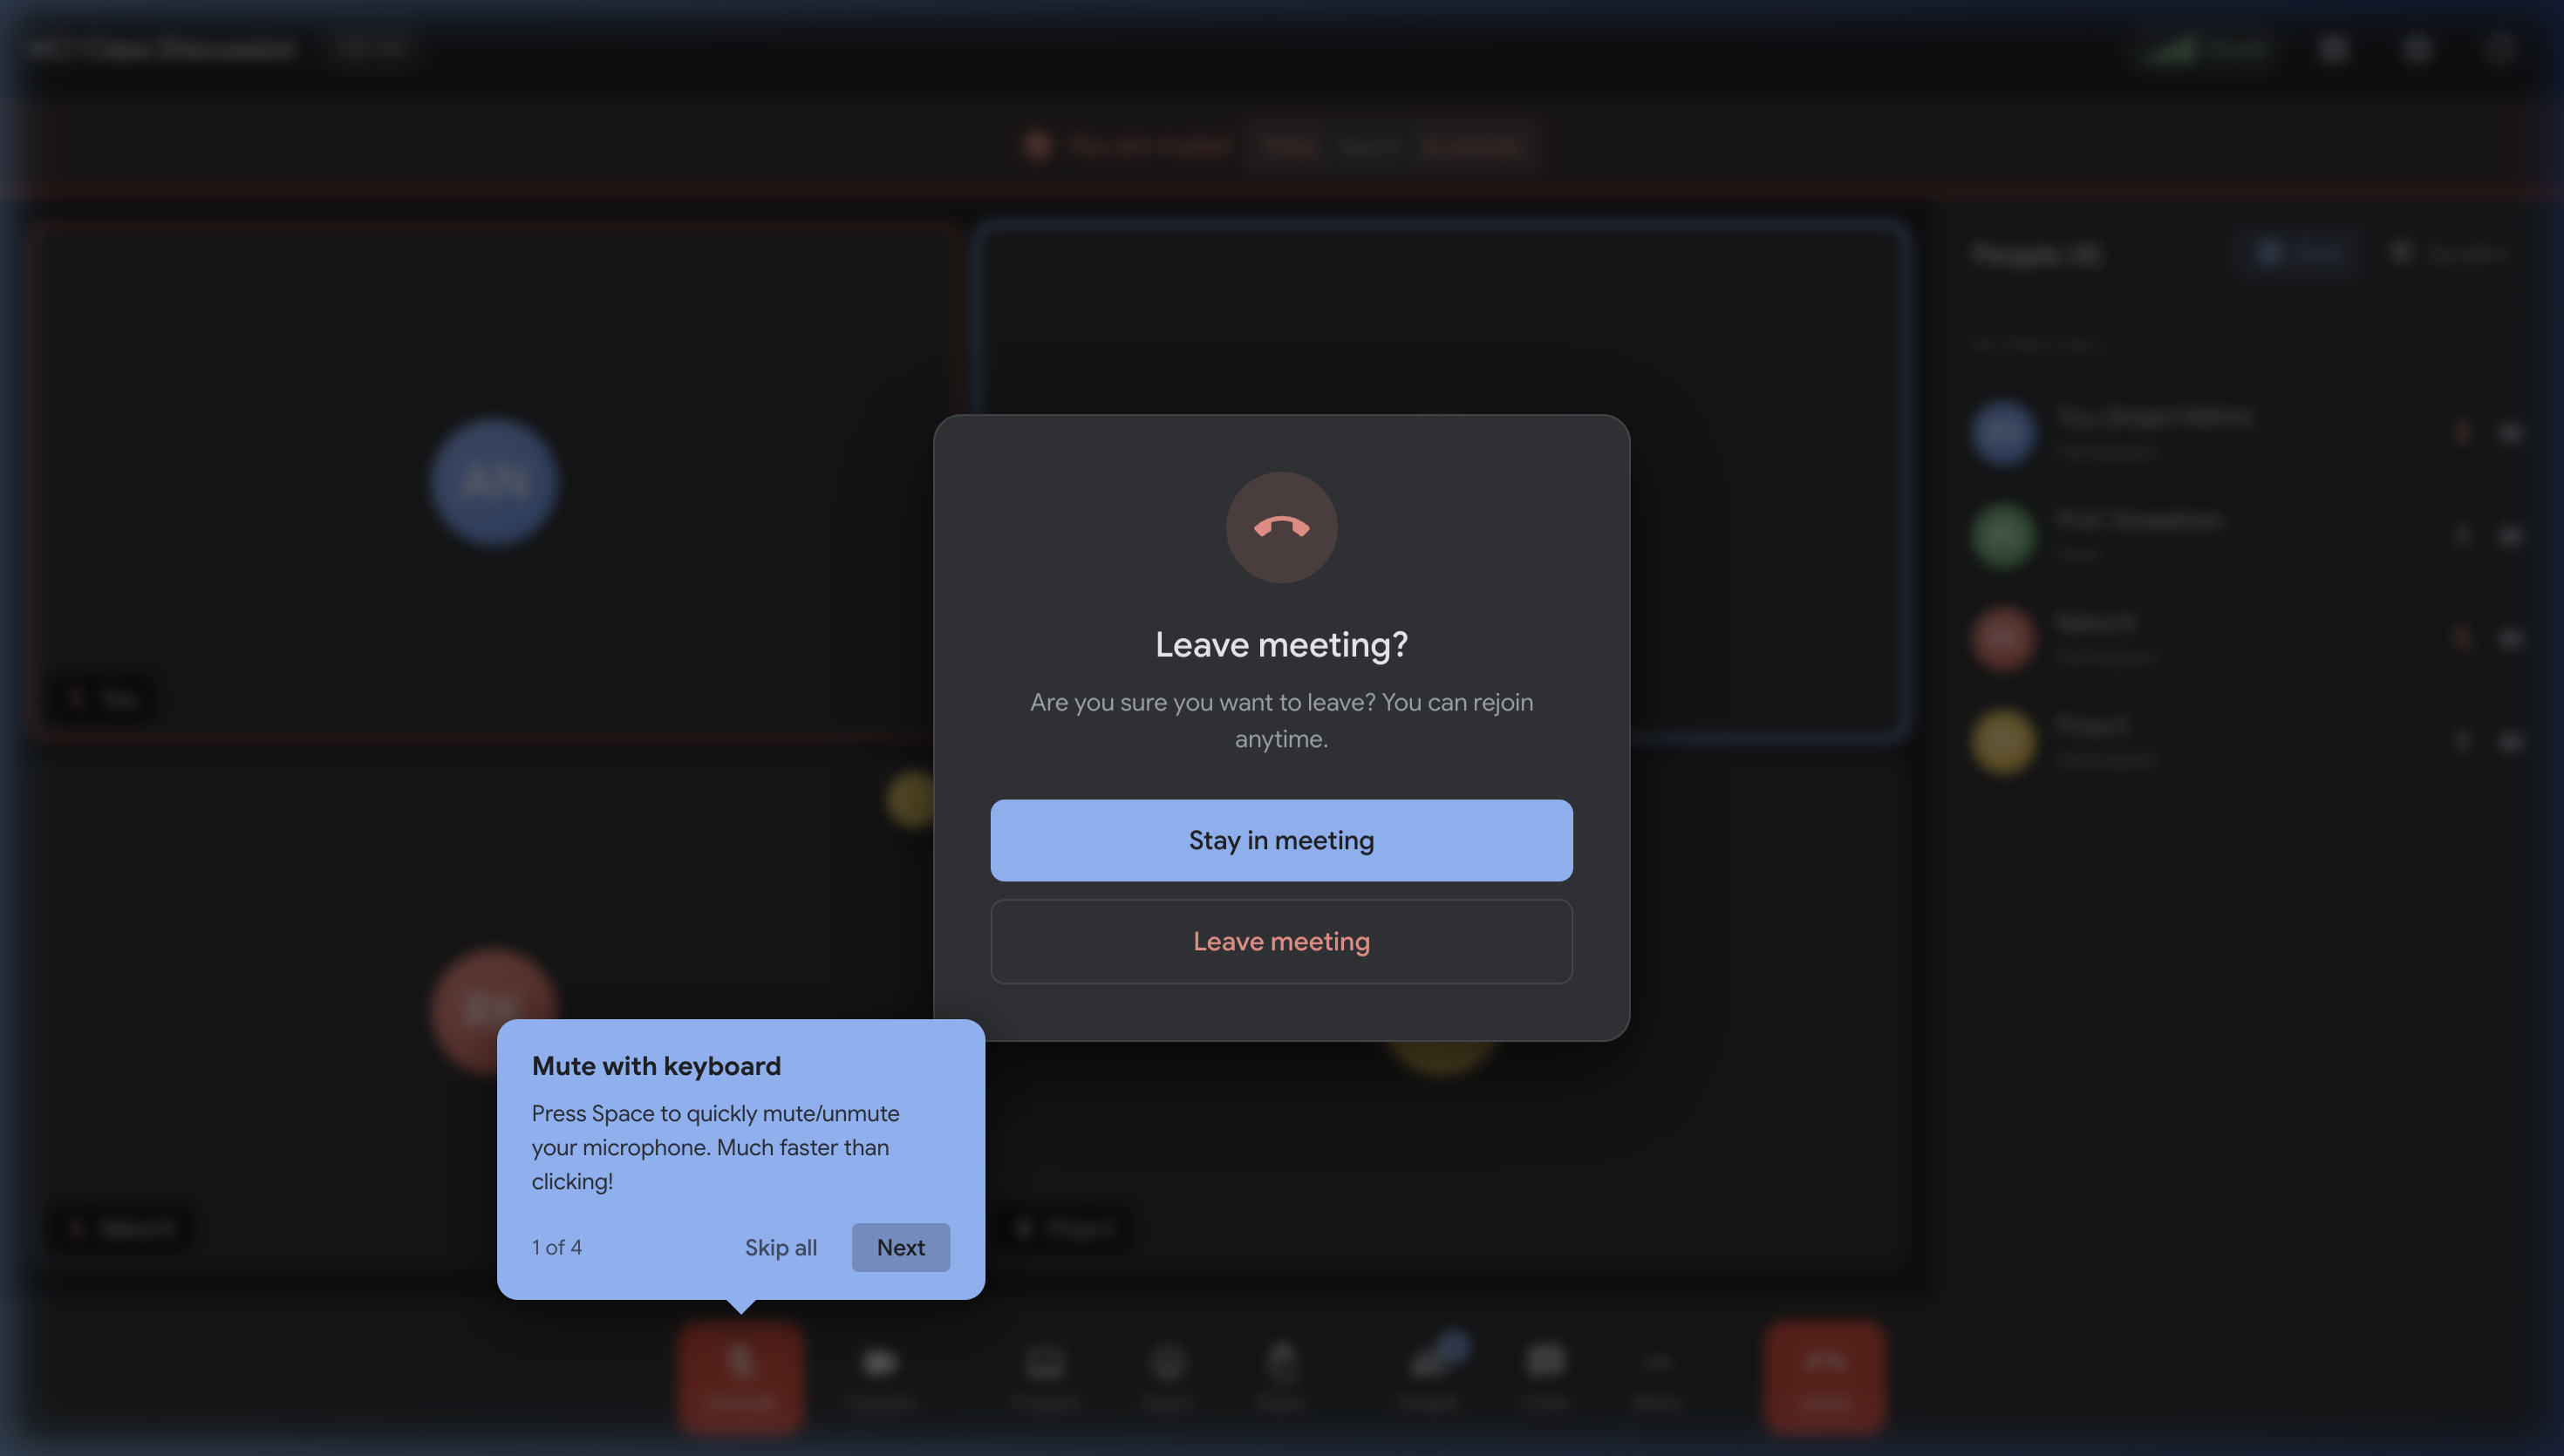
\includegraphics[width=0.85\textwidth]{images/leave_confirm.png}
    \caption{Hierarchy \& Contrast: The destructive (Leave Call) action forces a modality break before the engagement scores appear.}
\end{figure}

Following the confirmed disconnection, we utilize \textbf{Scale} to emphasize the "Meeting Streak" (Consistency), anchoring closure with positive reinforcement to drive habit loops, entirely abandoning the legacy blank exit screen.

\begin{figure}[H]
    \centering
    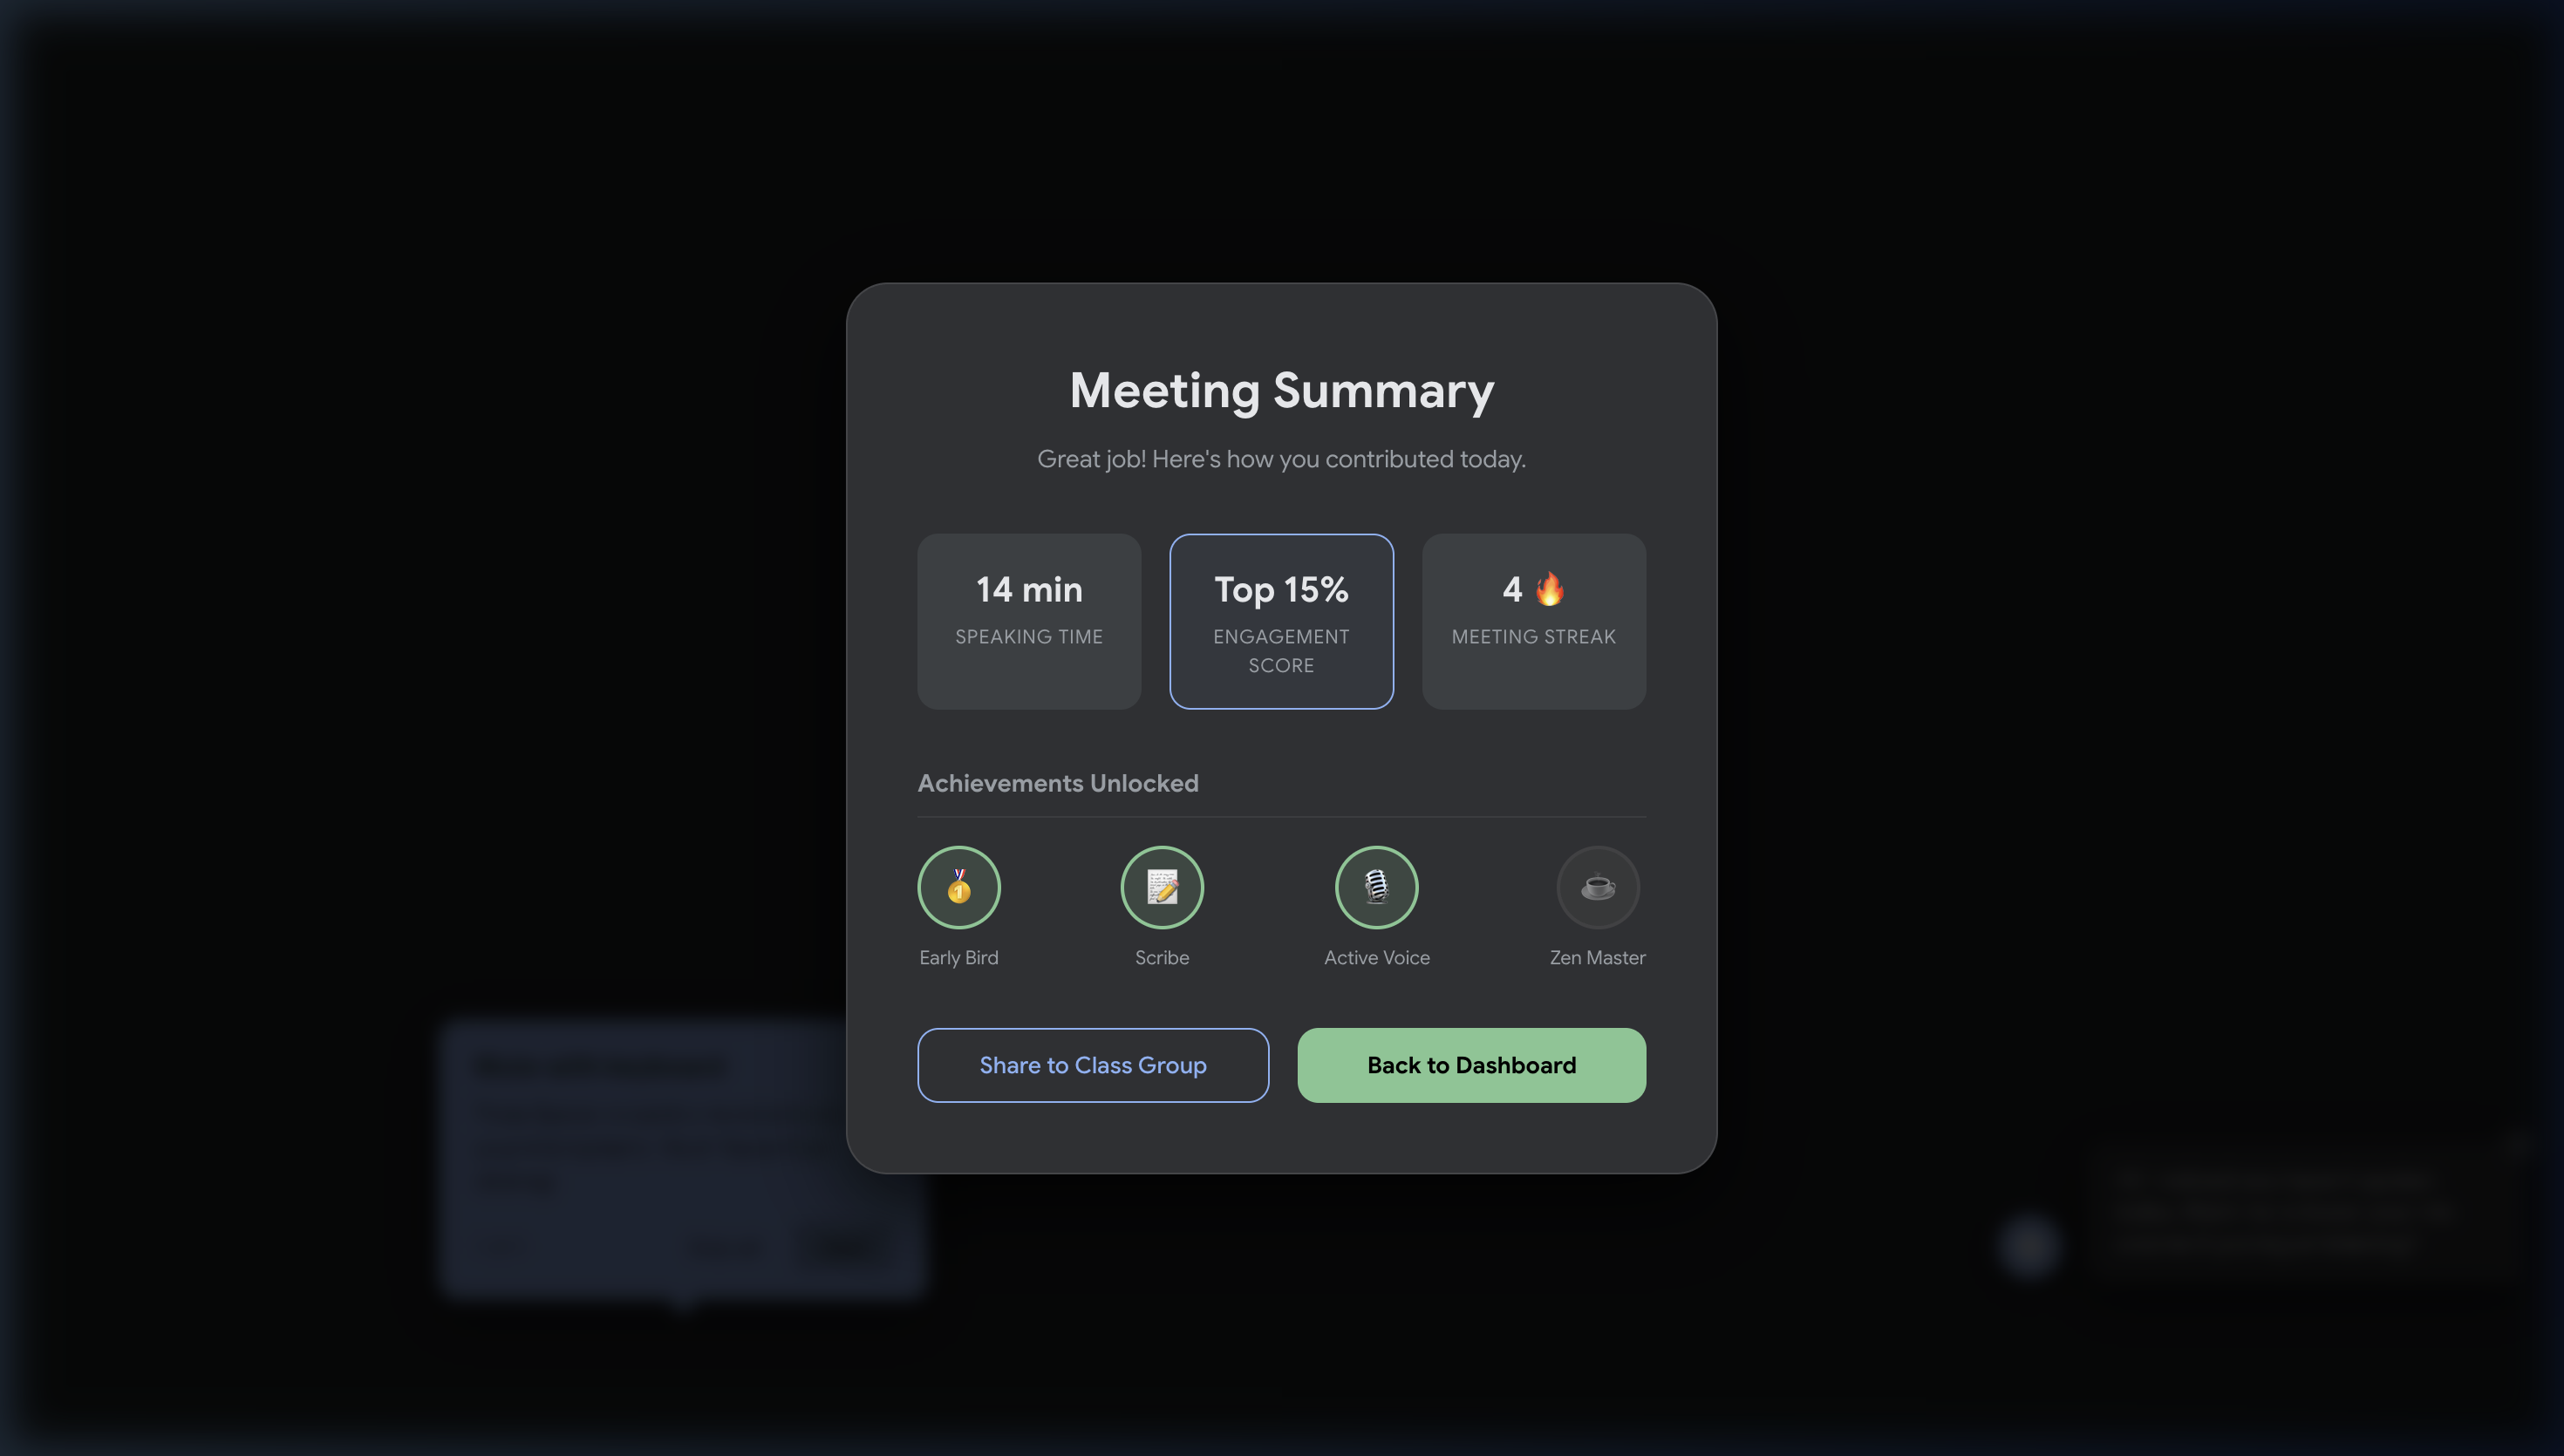
\includegraphics[width=0.7\textwidth]{images/gamification.png}
    \caption{Post-Meeting Gamification utilizing Scale to highlight Streaks.}
\end{figure}


\section{Conclusion}
Phase II actively marries deep behavioral psychology (Persuasion, Nudges) with concrete graphic design fundamentals (Unity, Hierarchical Contrast). Our high-fidelity implementations prove that virtual interfaces can simultaneously maintain structural usability and actively defend the user's cognitive wellbeing.

\end{document}
